\documentclass[10pt,a4paper,onecolumn]{article}
\usepackage{marginnote}
\usepackage{graphicx}
\usepackage{xcolor}
\usepackage{authblk,etoolbox}
\usepackage{titlesec}
\usepackage{calc}
\usepackage{tikz}
\usepackage{hyperref}
\hypersetup{colorlinks,breaklinks,
            urlcolor=[rgb]{0.0, 0.5, 1.0},
            linkcolor=[rgb]{0.0, 0.5, 1.0}}
\usepackage{caption}
\usepackage{tcolorbox}
\usepackage{amssymb,amsmath}
\usepackage{ifxetex,ifluatex}
\usepackage{seqsplit}
\usepackage{fixltx2e} % provides \textsubscript
\usepackage[
  backend=biber,
%  style=alphabetic,
%  citestyle=numeric
]{biblatex}
\bibliography{paper.bib}


% --- Page layout -------------------------------------------------------------
\usepackage[top=3.5cm, bottom=3cm, right=1.5cm, left=1.0cm,
            headheight=2.2cm, reversemp, includemp, marginparwidth=4.5cm]{geometry}

% --- Default font ------------------------------------------------------------
% \renewcommand\familydefault{\sfdefault}

% --- Style -------------------------------------------------------------------
\renewcommand{\bibfont}{\small \sffamily}
\renewcommand{\captionfont}{\small\sffamily}
\renewcommand{\captionlabelfont}{\bfseries}

% --- Section/SubSection/SubSubSection ----------------------------------------
\titleformat{\section}
  {\normalfont\sffamily\Large\bfseries}
  {}{0pt}{}
\titleformat{\subsection}
  {\normalfont\sffamily\large\bfseries}
  {}{0pt}{}
\titleformat{\subsubsection}
  {\normalfont\sffamily\bfseries}
  {}{0pt}{}
\titleformat*{\paragraph}
  {\sffamily\normalsize}


% --- Header / Footer ---------------------------------------------------------
\usepackage{fancyhdr}
\pagestyle{fancy}
\fancyhf{}
%\renewcommand{\headrulewidth}{0.50pt}
\renewcommand{\headrulewidth}{0pt}
\fancyhead[L]{\hspace{-0.75cm}\includegraphics[width=5.5cm]{/Library/Frameworks/R.framework/Versions/4.1/Resources/library/rticles/rmarkdown/templates/joss/resources/JOSS-logo.png}}
\fancyhead[C]{}
\fancyhead[R]{}
\renewcommand{\footrulewidth}{0.25pt}

\fancyfoot[L]{\footnotesize{\sffamily Liang et.
al., (2022). \texttt{ggmatplot}: An R package for data visualization on
wide-format
data. \textit{Journal of Open Source Software}, (), . \href{https://doi.org/}{https://doi.org/}}}


\fancyfoot[R]{\sffamily \thepage}
\makeatletter
\let\ps@plain\ps@fancy
\fancyheadoffset[L]{4.5cm}
\fancyfootoffset[L]{4.5cm}

% --- Macros ---------

\definecolor{linky}{rgb}{0.0, 0.5, 1.0}

\newtcolorbox{repobox}
   {colback=red, colframe=red!75!black,
     boxrule=0.5pt, arc=2pt, left=6pt, right=6pt, top=3pt, bottom=3pt}

\newcommand{\ExternalLink}{%
   \tikz[x=1.2ex, y=1.2ex, baseline=-0.05ex]{%
       \begin{scope}[x=1ex, y=1ex]
           \clip (-0.1,-0.1)
               --++ (-0, 1.2)
               --++ (0.6, 0)
               --++ (0, -0.6)
               --++ (0.6, 0)
               --++ (0, -1);
           \path[draw,
               line width = 0.5,
               rounded corners=0.5]
               (0,0) rectangle (1,1);
       \end{scope}
       \path[draw, line width = 0.5] (0.5, 0.5)
           -- (1, 1);
       \path[draw, line width = 0.5] (0.6, 1)
           -- (1, 1) -- (1, 0.6);
       }
   }

% --- Title / Authors ---------------------------------------------------------
% patch \maketitle so that it doesn't center
\patchcmd{\@maketitle}{center}{flushleft}{}{}
\patchcmd{\@maketitle}{center}{flushleft}{}{}
% patch \maketitle so that the font size for the title is normal
\patchcmd{\@maketitle}{\LARGE}{\LARGE\sffamily}{}{}
% patch the patch by authblk so that the author block is flush left
\def\maketitle{{%
  \renewenvironment{tabular}[2][]
    {\begin{flushleft}}
    {\end{flushleft}}
  \AB@maketitle}}
\makeatletter
\renewcommand\AB@affilsepx{ \protect\Affilfont}
%\renewcommand\AB@affilnote[1]{{\bfseries #1}\hspace{2pt}}
\renewcommand\AB@affilnote[1]{{\bfseries #1}\hspace{3pt}}
\makeatother
\renewcommand\Authfont{\sffamily\bfseries}
\renewcommand\Affilfont{\sffamily\small\mdseries}
\setlength{\affilsep}{1em}


\ifnum 0\ifxetex 1\fi\ifluatex 1\fi=0 % if pdftex
  \usepackage[T1]{fontenc}
  \usepackage[utf8]{inputenc}

\else % if luatex or xelatex
  \ifxetex
    \usepackage{mathspec}
  \else
    \usepackage{fontspec}
  \fi
  \defaultfontfeatures{Ligatures=TeX,Scale=MatchLowercase}

\fi
% use upquote if available, for straight quotes in verbatim environments
\IfFileExists{upquote.sty}{\usepackage{upquote}}{}
% use microtype if available
\IfFileExists{microtype.sty}{%
\usepackage{microtype}
\UseMicrotypeSet[protrusion]{basicmath} % disable protrusion for tt fonts
}{}

\usepackage{hyperref}
\hypersetup{unicode=true,
            pdftitle={ggmatplot: An R package for data visualization on wide-format data},
            pdfborder={0 0 0},
            breaklinks=true}
\urlstyle{same}  % don't use monospace font for urls
\usepackage{graphicx,grffile}
\makeatletter
\def\maxwidth{\ifdim\Gin@nat@width>\linewidth\linewidth\else\Gin@nat@width\fi}
\def\maxheight{\ifdim\Gin@nat@height>\textheight\textheight\else\Gin@nat@height\fi}
\makeatother
% Scale images if necessary, so that they will not overflow the page
% margins by default, and it is still possible to overwrite the defaults
% using explicit options in \includegraphics[width, height, ...]{}
\setkeys{Gin}{width=\maxwidth,height=\maxheight,keepaspectratio}
\IfFileExists{parskip.sty}{%
\usepackage{parskip}
}{% else
\setlength{\parindent}{0pt}
\setlength{\parskip}{6pt plus 2pt minus 1pt}
}
\setlength{\emergencystretch}{3em}  % prevent overfull lines
\setcounter{secnumdepth}{0}
% Redefines (sub)paragraphs to behave more like sections
\ifx\paragraph\undefined\else
\let\oldparagraph\paragraph
\renewcommand{\paragraph}[1]{\oldparagraph{#1}\mbox{}}
\fi
\ifx\subparagraph\undefined\else
\let\oldsubparagraph\subparagraph
\renewcommand{\subparagraph}[1]{\oldsubparagraph{#1}\mbox{}}
\fi

% Pandoc syntax highlighting
\usepackage{color}
\usepackage{fancyvrb}
\newcommand{\VerbBar}{|}
\newcommand{\VERB}{\Verb[commandchars=\\\{\}]}
\DefineVerbatimEnvironment{Highlighting}{Verbatim}{commandchars=\\\{\}}
% Add ',fontsize=\small' for more characters per line
\usepackage{framed}
\definecolor{shadecolor}{RGB}{248,248,248}
\newenvironment{Shaded}{\begin{snugshade}}{\end{snugshade}}
\newcommand{\AlertTok}[1]{\textcolor[rgb]{0.94,0.16,0.16}{#1}}
\newcommand{\AnnotationTok}[1]{\textcolor[rgb]{0.56,0.35,0.01}{\textbf{\textit{#1}}}}
\newcommand{\AttributeTok}[1]{\textcolor[rgb]{0.77,0.63,0.00}{#1}}
\newcommand{\BaseNTok}[1]{\textcolor[rgb]{0.00,0.00,0.81}{#1}}
\newcommand{\BuiltInTok}[1]{#1}
\newcommand{\CharTok}[1]{\textcolor[rgb]{0.31,0.60,0.02}{#1}}
\newcommand{\CommentTok}[1]{\textcolor[rgb]{0.56,0.35,0.01}{\textit{#1}}}
\newcommand{\CommentVarTok}[1]{\textcolor[rgb]{0.56,0.35,0.01}{\textbf{\textit{#1}}}}
\newcommand{\ConstantTok}[1]{\textcolor[rgb]{0.00,0.00,0.00}{#1}}
\newcommand{\ControlFlowTok}[1]{\textcolor[rgb]{0.13,0.29,0.53}{\textbf{#1}}}
\newcommand{\DataTypeTok}[1]{\textcolor[rgb]{0.13,0.29,0.53}{#1}}
\newcommand{\DecValTok}[1]{\textcolor[rgb]{0.00,0.00,0.81}{#1}}
\newcommand{\DocumentationTok}[1]{\textcolor[rgb]{0.56,0.35,0.01}{\textbf{\textit{#1}}}}
\newcommand{\ErrorTok}[1]{\textcolor[rgb]{0.64,0.00,0.00}{\textbf{#1}}}
\newcommand{\ExtensionTok}[1]{#1}
\newcommand{\FloatTok}[1]{\textcolor[rgb]{0.00,0.00,0.81}{#1}}
\newcommand{\FunctionTok}[1]{\textcolor[rgb]{0.00,0.00,0.00}{#1}}
\newcommand{\ImportTok}[1]{#1}
\newcommand{\InformationTok}[1]{\textcolor[rgb]{0.56,0.35,0.01}{\textbf{\textit{#1}}}}
\newcommand{\KeywordTok}[1]{\textcolor[rgb]{0.13,0.29,0.53}{\textbf{#1}}}
\newcommand{\NormalTok}[1]{#1}
\newcommand{\OperatorTok}[1]{\textcolor[rgb]{0.81,0.36,0.00}{\textbf{#1}}}
\newcommand{\OtherTok}[1]{\textcolor[rgb]{0.56,0.35,0.01}{#1}}
\newcommand{\PreprocessorTok}[1]{\textcolor[rgb]{0.56,0.35,0.01}{\textit{#1}}}
\newcommand{\RegionMarkerTok}[1]{#1}
\newcommand{\SpecialCharTok}[1]{\textcolor[rgb]{0.00,0.00,0.00}{#1}}
\newcommand{\SpecialStringTok}[1]{\textcolor[rgb]{0.31,0.60,0.02}{#1}}
\newcommand{\StringTok}[1]{\textcolor[rgb]{0.31,0.60,0.02}{#1}}
\newcommand{\VariableTok}[1]{\textcolor[rgb]{0.00,0.00,0.00}{#1}}
\newcommand{\VerbatimStringTok}[1]{\textcolor[rgb]{0.31,0.60,0.02}{#1}}
\newcommand{\WarningTok}[1]{\textcolor[rgb]{0.56,0.35,0.01}{\textbf{\textit{#1}}}}

% tightlist command for lists without linebreak
\providecommand{\tightlist}{%
  \setlength{\itemsep}{0pt}\setlength{\parskip}{0pt}}


% Pandoc citation processing
\newlength{\cslhangindent}
\setlength{\cslhangindent}{1.5em}
\newlength{\csllabelwidth}
\setlength{\csllabelwidth}{3em}
\newlength{\cslentryspacingunit} % times entry-spacing
\setlength{\cslentryspacingunit}{\parskip}
% for Pandoc 2.8 to 2.10.1
\newenvironment{cslreferences}%
  {}%
  {\par}
% For Pandoc 2.11+
\newenvironment{CSLReferences}[2] % #1 hanging-ident, #2 entry spacing
 {% don't indent paragraphs
  \setlength{\parindent}{0pt}
  % turn on hanging indent if param 1 is 1
  \ifodd #1
  \let\oldpar\par
  \def\par{\hangindent=\cslhangindent\oldpar}
  \fi
  % set entry spacing
  \setlength{\parskip}{#2\cslentryspacingunit}
 }%
 {}
\usepackage{calc}
\newcommand{\CSLBlock}[1]{#1\hfill\break}
\newcommand{\CSLLeftMargin}[1]{\parbox[t]{\csllabelwidth}{#1}}
\newcommand{\CSLRightInline}[1]{\parbox[t]{\linewidth - \csllabelwidth}{#1}\break}
\newcommand{\CSLIndent}[1]{\hspace{\cslhangindent}#1}

\usepackage{booktabs}
\usepackage{longtable}
\usepackage{array}
\usepackage{multirow}
\usepackage{wrapfig}
\usepackage{float}
\usepackage{colortbl}
\usepackage{pdflscape}
\usepackage{tabu}
\usepackage{threeparttable}
\usepackage{threeparttablex}
\usepackage[normalem]{ulem}
\usepackage{makecell}
\usepackage{xcolor}

\title{\texttt{ggmatplot}: An R package for data visualization on
wide-format data}

        \author[1]{Xuan Liang}
          \author[1]{Francis K. C. Hui}
          \author[2]{Dilinie Seimon}
          \author[2]{Emi Tanaka}
    
      \affil[1]{Research School of Finance, Actuarial Studies and
Statistics, The Australian National University}
      \affil[2]{Department of Econometrics and Business Statistics,
Monash University}
  \date{\vspace{-5ex}}

\begin{document}
\maketitle

\marginpar{
  %\hrule
  \sffamily\small

  {\bfseries DOI:} \href{https://doi.org/}{\color{linky}{}}

  \vspace{2mm}

  {\bfseries Software}
  \begin{itemize}
    \setlength\itemsep{0em}
    \item \href{}{\color{linky}{Review}} \ExternalLink
    \item \href{}{\color{linky}{Repository}} \ExternalLink
    \item \href{}{\color{linky}{Archive}} \ExternalLink
  \end{itemize}

  \vspace{2mm}

  {\bfseries Submitted:} \\
  {\bfseries Published:} 

  \vspace{2mm}
  {\bfseries License}\\
  Authors of papers retain copyright and release the work under a Creative Commons Attribution 4.0 International License (\href{http://creativecommons.org/licenses/by/4.0/}{\color{linky}{CC-BY}}).
}

\hypertarget{summary}{%
\section{Summary}\label{summary}}

The layered grammar of graphics (Wickham, 2010), implemented as the
\texttt{ggplot2} package (Wickham, 2016) in the statistical language R
(R Core Team, 2021), is a powerful and popular tool to create versatile
statistical graphics. However, this graphical system requires input data
to be organised in a manner that a data column is mapped to an aesthetic
element (e.g.~x-coordinate, y-coordinate, color, size), which creates
friction in constructing plots with an aesthetic element that span
multiple columns in the original data by requiring users to re-organise
the data.\\

\emph{Regarding Francis' question, I don't know if the long format or
wide format data are well defined in the literature. If it is, we
definitely can mention it. If not, do we need to define it? --commented
by XL}

The \texttt{ggmatplot}, built upon \texttt{ggplot2}, is an R-package
that allows quick plotting across the columns of matrices or data with
the result returned as a \texttt{ggplot} object. The package is inspired
by the function \texttt{matplot()} in the core R \texttt{graphics}
system -- as such, \texttt{ggmatplot} may be considered as a
\texttt{ggplot} version of \texttt{matplot} with the benefits of
customising the plots as any other \texttt{ggplot} objects via
\texttt{ggplot2} functions, as well as offering several other plotting
types that are not immediately available from \texttt{matplot} directly,
such as comparative violin plots.

\hypertarget{statement-of-need}{%
\section{Statement of need}\label{statement-of-need}}

Input data to construct plots with \texttt{ggplot2} require data to be
organised in a manner that maps data columns to aesthetic elements. This
generally works well where data is tidied in a long rectangular form,
often referred to as ``tidy data'' (Wickham, 2014), where each row
represents an observational unit, each column represents a variable, and
each cell represents a value. In some cases, what constitutes a variable
(or observational unit), and hence a column (or row), in tidy data can
be dependent upon interpretation or downstream interest (e.g.~Tables
\ref{tab:tab1} and \ref{tab:tab2} can be both considered as tidy data),
but a clear violation of tidy data principles is when the column names
contain data values, e.g.~\emph{Table \ref{tab:tab3} contain the name of
the species across a number of column names.} THIS IS WRONG? THERE ARE
NO SPECIES HERE?

\begin{table}

\caption{\label{tab:tab1}Restaurant rating data in "tidy" form. The first column shows the restaurant ID, and the next four columns show the average ratings (out of 5) for food, service, ambience and overall, respectively.}
\centering
\begin{tabular}[t]{lrrrr}
\toprule
\multicolumn{1}{c}{ } & \multicolumn{4}{c}{Average rating} \\
\cmidrule(l{3pt}r{3pt}){2-5}
Restaurant & Food & Service & Ambience & Overall\\
\midrule
R1 & 4.3 & 3.4 & 4.3 & 4.9\\
R2 & 4.3 & 5.0 & 4.5 & 4.4\\
R3 & 3.2 & 4.4 & 5.0 & 3.0\\
R4 & 2.3 & 4.6 & 4.4 & 3.8\\
R5 & 3.9 & 4.8 & 4.2 & 3.3\\
\bottomrule
\end{tabular}
\end{table}

\begin{table}

\caption{\label{tab:tab2}Another form for the restaurant rating data in Table \ref{tab:tab1}. In Wickham (2014), this format is called the "molten" data.}
\centering
\begin{tabular}[t]{llr}
\toprule
Restauant & Rating type & Average rating\\
\midrule
R1 & food & 4.3\\
R1 & service & 3.4\\
R1 & ambience & 4.3\\
R1 & overall & 4.9\\
R2 & food & 4.3\\
R2 & service & 5.0\\
R2 & ambience & 4.5\\
R2 & overall & 4.4\\
R3 & food & 3.2\\
R3 & service & 4.4\\
R3 & ambience & 5.0\\
R3 & overall & 3.0\\
R4 & food & 2.3\\
R4 & service & 4.6\\
R4 & ambience & 4.4\\
R4 & overall & 3.8\\
R5 & food & 3.9\\
R5 & service & 4.8\\
R5 & ambience & 4.2\\
R5 & overall & 3.3\\
\bottomrule
\end{tabular}
\end{table}

\begin{table}

\caption{\label{tab:tab3}The first 6 rows and 11 columns of the snowfall data for Grand Rapids, Michigan in the R pacakge   exttt{mosaicData} (Prium, Kaplan \& Horton, 2021).}
\centering
\begin{tabular}[t]{rrrrrrrrrrr}
\toprule
SeasonStart & SeasonEnd & Jul & Aug & Sep & Oct & Nov & Dec & Jan & Feb & Mar\\
\midrule
1893 & 1894 & 0 & 0 & 0 & 0.0 & 8.0 & 24.9 & 12.5 & 6.8 & 4.8\\
1894 & 1895 & 0 & 0 & 0 & 0.0 & 7.5 & 5.3 & 21.5 & 8.0 & 22.5\\
1895 & 1896 & 0 & 0 & 0 & 0.4 & 23.2 & 15.0 & . & 8.5 & 2.0\\
1896 & 1897 & 0 & 0 & 0 & 0.2 & 8.0 & 8.0 & 4.9 & 11.2 & 12.0\\
1897 & 1898 & 0 & 0 & 0 & 0.0 & 1.4 & 8.0 & 15.5 & 29.5 & 0.0\\
1898 & 1899 & 0 & 0 & 0 & 0.0 & 18.5 & 18.0 & 20 & 3.4 & 16.0\\
\bottomrule
\end{tabular}
\end{table}

The organisation of the data is largely dependent on the downstream
analysis, and there is no one correct way to do this. Some forms of
multivariate data, e.g.~Table \ref{tab:tab3}, are prevalent in many
scientific fields because it aligns with the input data for a particular
modelling software, and/or the format is more convenient for input or
view of the data in spreadsheet format (say). Unfortunately, this format
is not consistent with the required format for \texttt{ggplot2}, and
consequently plotting with \texttt{ggplot2} interrupts the workflow of a
user that is trying to quickly visualise these types of data (as part of
their exploratory data analysis, say). The \texttt{ggmatplot} R-package
seeks to provide a solution to this common friction in producing plots
with \texttt{ggplot2}.

\hypertarget{examples}{%
\section{Examples}\label{examples}}

In this section, we demonstrate the use of the \texttt{ggmatplot}
package and contrast the specification with \texttt{ggplot2} after data
wrangling using \texttt{dplyr} and \texttt{tidyr} (Wickham et al.,
2019). We will use the example data in Tables \ref{tab:tab1} and
\ref{tab:tab3}, which are stored in the objects \texttt{wide\_df} and
\texttt{SnowGR}, respectively.

\hypertarget{example-1}{%
\subsection{Example 1}\label{example-1}}

The code below constructs a line plot (superimposed with a point) of the
various types (food, service and ambience) of ratings, contained in
columns 2 to 4 of \texttt{wide\_df}, against the overall restaurant
rating in column 5 of \texttt{wide\_df} as shown in Figure 1.

\emph{In example 1, should X lab be restaurant or rating? The one made
by ggmatplot is different from the one made by ggplot. Currently, the
plot does not show a clear relationship between various types and the
overall rating. Is it better to compare the ratings among restaurants?
-- commented by XL}

\begin{Shaded}
\begin{Highlighting}[]
\FunctionTok{library}\NormalTok{(ggmatplot)}
\FunctionTok{ggmatplot}\NormalTok{(}\AttributeTok{x =}\NormalTok{ wide\_df[, }\DecValTok{2}\SpecialCharTok{:}\DecValTok{4}\NormalTok{], }\AttributeTok{y =}\NormalTok{ wide\_df[, }\DecValTok{5}\NormalTok{], }\AttributeTok{plot\_type =} \StringTok{"both"}\NormalTok{,}
          \AttributeTok{xlab =} \StringTok{"Rating"}\NormalTok{,  }\AttributeTok{ylab =} \StringTok{"Overall rating"}\NormalTok{, }\AttributeTok{legend\_title =} \StringTok{"Type"}\NormalTok{) }
\end{Highlighting}
\end{Shaded}

\begin{figure}
\centering
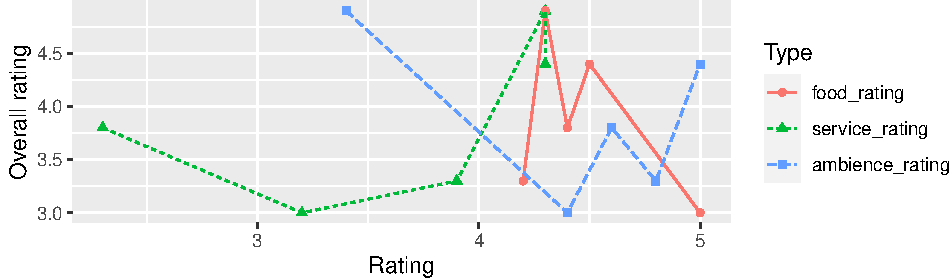
\includegraphics{paper_files/figure-latex/matplot2-1.pdf}
\caption{Line plot of the food, service and ambience rating against the
overall restaurant rating.}
\end{figure}

In contrast to the above, using \texttt{ggplot2} alone, the data must be
wrangled to a long form first before plotting, as exemplified in the
code below, in order to obtain the same result as Figure 1. This adds a
small, but noticeable, friction to the workflow for the practitioner
that is looking to promptly explore their data.

\begin{Shaded}
\begin{Highlighting}[]
\FunctionTok{library}\NormalTok{(ggplot2)}
\FunctionTok{library}\NormalTok{(tidyr) }\CommentTok{\# or library(tidyverse)}
\NormalTok{wide\_df }\SpecialCharTok{\%\textgreater{}\%} 
  \FunctionTok{select}\NormalTok{(}\FunctionTok{contains}\NormalTok{(}\StringTok{"rating"}\NormalTok{)) }\SpecialCharTok{\%\textgreater{}\%} 
  \FunctionTok{pivot\_longer}\NormalTok{(}\SpecialCharTok{{-}}\NormalTok{overall\_rating, }
               \AttributeTok{names\_to =} \StringTok{"rating\_type"}\NormalTok{,}
               \AttributeTok{values\_to =} \StringTok{"rating"}\NormalTok{) }\SpecialCharTok{\%\textgreater{}\%} 
  \FunctionTok{ggplot}\NormalTok{(}\FunctionTok{aes}\NormalTok{(rating, overall\_rating, }\AttributeTok{color =}\NormalTok{ rating\_type)) }\SpecialCharTok{+} 
  \FunctionTok{geom\_point}\NormalTok{(}\FunctionTok{aes}\NormalTok{(}\AttributeTok{shape =}\NormalTok{ rating\_type)) }\SpecialCharTok{+}
  \FunctionTok{geom\_line}\NormalTok{(}\FunctionTok{aes}\NormalTok{(}\AttributeTok{group =}\NormalTok{ rating\_type, }\AttributeTok{linetype =}\NormalTok{ rating\_type)) }\SpecialCharTok{+}
  \FunctionTok{labs}\NormalTok{(}\AttributeTok{x =} \StringTok{"Restaurant"}\NormalTok{, }\AttributeTok{y =} \StringTok{"Rating"}\NormalTok{, }
       \AttributeTok{color =} \StringTok{"Type"}\NormalTok{, }\AttributeTok{linetype =} \StringTok{"Type"}\NormalTok{, }\AttributeTok{shape =} \StringTok{"Type"}\NormalTok{)}
\end{Highlighting}
\end{Shaded}

\hypertarget{example-2}{%
\subsection{Example 2}\label{example-2}}

The example code draws the boxplot of each column of amount of snowfall
across months in the \texttt{SnowGR} data as shown in Figure 2. As the
resulting object is a \texttt{ggplot} object, the user can leverage the
\texttt{ggplot} functions to modify the output (e.g.~removal of the
legend). CAN WE \texttt{fct\_inorder} SO THAT THE MONTHS APPEAR IN ORDER
OF THEIR COLUMN NAMES? EMI HAS ALREADY PICKED THIS UP AS AN
ISSUE\ldots{}

\emph{Now the color and fill has been removed for boxplot. So by
default, there is no legend. We may need to change the demonstration of
Example 2. -- commented by XL} \emph{Another question is that only the
github version has such setting. Do I need to submit the new version to
CRAN? -- commented by XL}

\begin{Shaded}
\begin{Highlighting}[]
\FunctionTok{library}\NormalTok{(ggmatplot)}
\FunctionTok{ggmatplot}\NormalTok{(}\AttributeTok{x =}\NormalTok{ SnowGR[, }\DecValTok{3}\SpecialCharTok{:}\DecValTok{14}\NormalTok{], }\AttributeTok{plot\_type =} \StringTok{"boxplot"}\NormalTok{,}
          \AttributeTok{xlab =} \StringTok{"Month"}\NormalTok{,  }\AttributeTok{ylab =} \StringTok{"Snowfall"}\NormalTok{) }\SpecialCharTok{+}
  \FunctionTok{guides}\NormalTok{(}\AttributeTok{color =} \StringTok{"none"}\NormalTok{, }\AttributeTok{fill =} \StringTok{"none"}\NormalTok{)}
\end{Highlighting}
\end{Shaded}

\begin{figure}
\centering
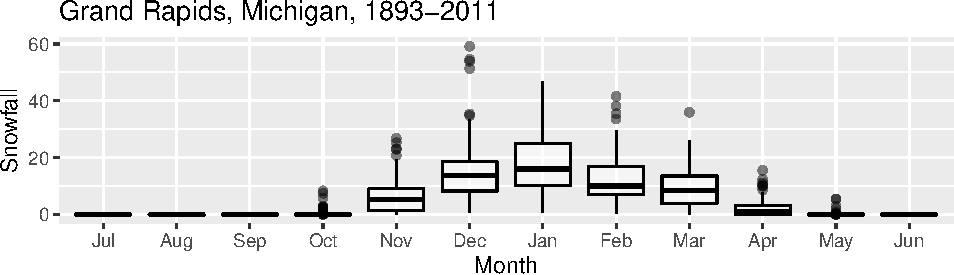
\includegraphics{paper_files/figure-latex/matplot3-1.pdf}
\caption{The distribution of the amount of snowfall at Grand Rapids,
Michigan, across months from 1893-2011.}
\end{figure}

The equivalent code for the above to produce Figure 2 without using
\texttt{ggmatplot} is given below. Again, we observe a slight but
non-negligible friction in putting the data in the right format prior to
plotting. The original wide data format like those shown in Table
\ref{tab:tab3} is common in the environmental sciences among other
disciplines, and thus an analyst who has to repeat these tasks can
benefit from a quick approach as \texttt{ggmatplot} offers.

\begin{Shaded}
\begin{Highlighting}[]
\FunctionTok{library}\NormalTok{(ggplot2)}
\FunctionTok{library}\NormalTok{(tidyr) }\CommentTok{\# or library(tidyverse)}
\NormalTok{SnowGR }\SpecialCharTok{\%\textgreater{}\%} 
  \FunctionTok{pivot\_longer}\NormalTok{(Jul}\SpecialCharTok{:}\NormalTok{Jun, }
               \AttributeTok{names\_to =} \StringTok{"Month"}\NormalTok{,}
               \AttributeTok{values\_to =} \StringTok{"Snowfall"}\NormalTok{) }\SpecialCharTok{\%\textgreater{}\%} 
  \FunctionTok{ggplot}\NormalTok{(}\FunctionTok{aes}\NormalTok{(Month, Snowfall)) }\SpecialCharTok{+} 
  \FunctionTok{geom\_boxplot}\NormalTok{(}\FunctionTok{aes}\NormalTok{(}\AttributeTok{color =}\NormalTok{ Month, }\AttributeTok{fill =}\NormalTok{ Month), }\AttributeTok{alpha =} \FloatTok{0.5}\NormalTok{) }\SpecialCharTok{+}
  \FunctionTok{guides}\NormalTok{(}\AttributeTok{color =} \StringTok{"none"}\NormalTok{, }\AttributeTok{fill =} \StringTok{"none"}\NormalTok{)}
\end{Highlighting}
\end{Shaded}

WOULD IT BENEFIT FROM ALSO SHOWING A PLOT THAT BASE MATPLOT CAN NOT? THE
ABOVE CAN BE DONE BY APPLY \texttt{boxplot}, AND HENCE WHY I WROTE
VIOLIN PLOT AT THE BEGINNING AS IT IS NOT AVAILABLE AT LEAST IN CORE R?

\emph{The other option is the density plot which can not be done by
matplot--commented by XL. But since there are too many months, it might
not be a good idea. -- commented by XL}

\hypertarget{discussion}{%
\section{Discussion}\label{discussion}}

The \texttt{ggmatplot} R-package provides a solution to a common
friction encountered when wanting to quickly plot multivariate data,
where the primary interest is mapping the column names as an aesthetic
element. While an excellent start, we also acknowledge that solution
provided is a recipe-driven approach, where the user can only produce
plot types as many there are included in the \texttt{plot\_type} option.
Future developments of the package could benefit from using a grammar
approach, like in Wilkinson (2005) and Wickham (2010), where plot types
can be extensible.

\hypertarget{acknowledgements}{%
\section{Acknowledgements}\label{acknowledgements}}

FKCH was supported by an Australian Research Council Discovery
Fellowship DE200100435.

\hypertarget{references}{%
\section*{References}\label{references}}
\addcontentsline{toc}{section}{References}

\hypertarget{refs}{}
\begin{CSLReferences}{1}{0}
\leavevmode\hypertarget{ref-mosaicData}{}%
Pruim, R., Kaplan, D., \& Horton, N. (2021). \emph{mosaicData: Project
MOSAIC data sets}. Retrieved from
\url{https://CRAN.R-project.org/package=mosaicData}

\leavevmode\hypertarget{ref-rstats}{}%
R Core Team. (2021). \emph{R: A language and environment for statistical
computing}. Vienna, Austria: R Foundation for Statistical Computing.
Retrieved from \url{https://www.R-project.org/}

\leavevmode\hypertarget{ref-Wickham2010-kt}{}%
Wickham, H. (2010). A layered grammar of graphics. \emph{Journal of
computational and graphical statistics: a joint publication of American
Statistical Association, Institute of Mathematical Statistics, Interface
Foundation of North America}.

\leavevmode\hypertarget{ref-Wickham2014-gy}{}%
Wickham, H. (2014). Tidy data. \emph{Journal of Statistical Software},
\emph{59}(10), 1--23.
doi:\href{https://doi.org/10.18637/jss.v059.i10}{10.18637/jss.v059.i10}

\leavevmode\hypertarget{ref-Wickham2016}{}%
Wickham, H. (2016). \emph{ggplot2: Elegant graphics for data analysis}.
Springer-Verlag New York. Retrieved from
\url{https://ggplot2.tidyverse.org}

\leavevmode\hypertarget{ref-Wickham2019}{}%
Wickham, H., Averick, M., Bryan, J., Chang, W., McGowan, L. D.,
François, R., Grolemund, G., et al. (2019). Welcome to the {tidyverse}.
\emph{Journal of Open Source Software}, \emph{4}(43), 1686.
doi:\href{https://doi.org/10.21105/joss.01686}{10.21105/joss.01686}

\leavevmode\hypertarget{ref-Wilkinson2005-oz}{}%
Wilkinson, L. (2005). \emph{The grammar of graphics}. Springer.

\end{CSLReferences}

\end{document}
